\section{Gestion des cours de la bourse : Yahoo! Finance}

Dans le cadre de ce projet nous avons besoin de connaître les cours des indices et des actions pour pouvoir permettre au joueur de faire des paris sur ce qu'il va se passer.

\subsection{Présentation}

Yahoo! Finance est un site internet du groupe Yahoo! qui délivre de nombreuses informations dans le domaine de la finance. Ainsi, nous retrouvons une section actualité qui nous permet d'avoir un rapide coup d’œil sur les divers articles de journaux en rapport avec l'économie. Dans la partie vidéo le principe est le même sauf que les actualités sont sous forme de vidéos. \\

Yahoo propose de visualiser de nombreuses informations en rapport avec les cours ou indices. \\

Par exemple, pour l'indice du CAC40 on retrouve sa valeur ainsi que sa variation par rapport à la dernière session. On a accès à la dernière valeur de clôture ainsi que la valeur à l'ouverture. Un graphique représente l'évolution du prix de l'indice depuis l'ouverture de la session. Nous avons également accès aux articles concernant le CAC40 dans la presse écrite, aux composants du CAC40 ainsi qu'aux prix historiques (valeur ouverture, fermeture, haut, bas sur la période désirée). \\


Pour un indice, ACCOR S.A dans notre exemple la page se présente comme suit : \\
\begin{figure}[H]
  \center
  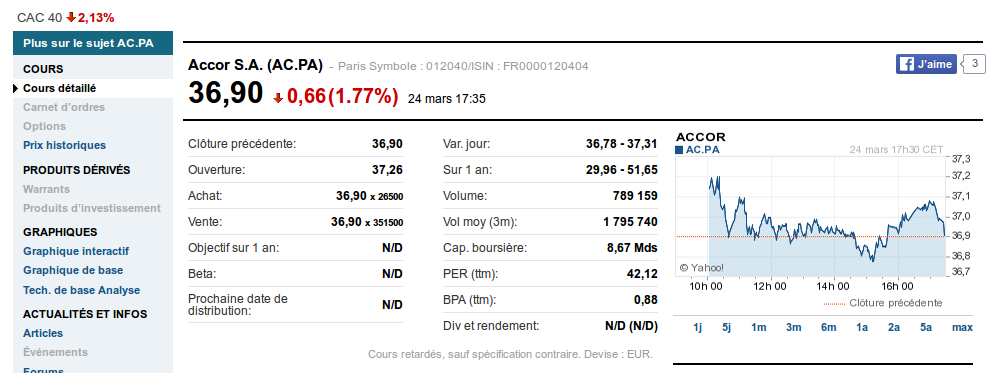
\includegraphics[scale=0.4]{../graph/yahoo.png} \\
  \caption{Visualisation du site Yahoo! Finance}
\end{figure}
Nous retrouvons les prix historiques (ce qui nous intéresse) ainsi que d'autres informations concernant le cours. 

\subsection{Principe du téléchargement}

Nous avons vu dans la partie précédente que nous avions accès à l'historique des cours pour les indices et les cours. Nous avons la possibilité de télécharger ces cours au format CSV. La chose intéressante à étudier est la construction de l'URL qui permet d'effectuer ce téléchargement. \\ 

Par exemple, regardons l'URL pour télécharger le cours d'IBM entre le 01 janvier 2016 et le 01 février : 
\begin{lstlisting}
real-chart.finance.yahoo.com/table.csv?s=IBM&a=00&b=1&c=2016&d=01&e=1&f=2016&g=d&ignore=.csv
\end{lstlisting}
Nous pouvons ainsi étudier la construction de l'URL qui sera la même pour télécharger chacun des cours. L'URL est construit de la manière suivante : 
\begin{itemize} 
\item "real-chart.finance.yahoo.com/table.csv?" une première partie fixe qui sera commune à tous les téléchargements 
\item "s=IBM" qui permet de savoir quel action/indice nous téléchargeons. Ici IBM correspond au code d'IBM sur la site Yahoo! Finance
\item "\&a=00\&b=1\&c=2016" correspond à la date à partir de laquelle nous souhaitons télécharger les valeurs, "a" correspond au mois (00 = janvier), b au jour, et c à l'année
\item "\&d=01\&e=1\&f=2016" correspond à la date jusqu'à laquelle nous souhaitons télécharger les valeurs, "d" correspond au mois (01 = février), e au jour, et f à l'année
\item "\&g=d" signifie que nous voulons télécharger les valeurs jour par jour, nous aurions pu choisir semaine par semaine ou mensuellement
\item "\&ignore=.csv" enfin cela signifie que nous voulons télécharger au format csv
\end{itemize}

Une fois cette remarque effectuée nous voyons que le code pour télécharger le cours est très simple : 

\begin{lstlisting}
//Construisons l'url de notre page
		//Chaque url permettant d'acceder aux cours de la bourse est construit de la meme maniere
String url="http://real-chart.finance.yahoo.com/table.csv?"+
		           "s="+code  //code correspondant a l'action
		           +"&a="+debut.get(Calendar.MONTH) //mois de debut 00=janvier, 01=fevrier, 02=mars...
		           +"&b="+debut.get(Calendar.DAY_OF_MONTH) //jour de debut
		           +"&c="+debut.get(Calendar.YEAR) //annee de debut
		           +"&d="+fin.get(Calendar.MONTH)
		           +"&e="+fin.get(Calendar.DAY_OF_MONTH)
		           +"&f="+fin.get(Calendar.YEAR)
		           +"&g=d" //On veut par jour
		           +"&ignore=.csv"; //au format csv;
		
		//Il ne nous reste plus qu'a nous connecter a l'url et copier les donnees
		try
		{
			URL yahooUrl = new URL(url);
			URLConnection donnee = yahooUrl.openConnection();
			Scanner entree = new Scanner(donnee.getInputStream());
			
			while(entree.hasNextLine()){
				String ligne = entree.nextLine();
				Traitement de la ligne
			}	
		}
		catch(Exception e)
		{
			System.err.println(e);
		}
\end{lstlisting} 